\documentclass{article}
\usepackage{amsmath,graphicx}
\begin{document}
\title{Summed self force is smooth}
\author{Steven Dorsher}
\maketitle

After taking the median, the maximum, and the minimum, but especially the median and maximum of a sorted list of the orders of finfs that do not produce nan's (I believe sorting by finf), the summed self force evolves smoothly. The minimum has a high relative error with features compared to the other two, which seem random and have a low relative error relative to each other. The two term and three term cases, for the median, have a relative error on the order of $10^{-4}$. I have tested the case where several lmins and lmaxes are run, and the average over that surface is taken. I am using the small region of lmins and lmaxes. the finfindex in fitcoefftable.py needs to be modified to run with the new bestfinfselector.py output, depending on whether a min, a max, or a median is chosen.  It would be ideal to make this a command line or script option.

\begin{figure}
  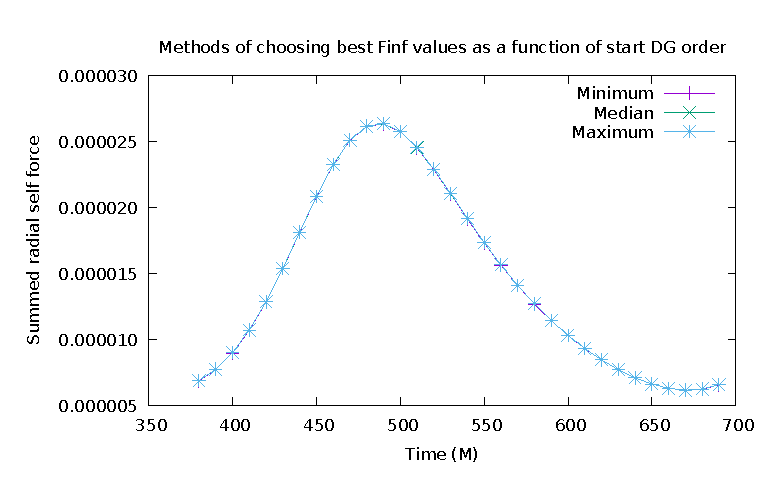
\includegraphics{bestfinfscriptplot}
\end{figure}

\begin{figure}
  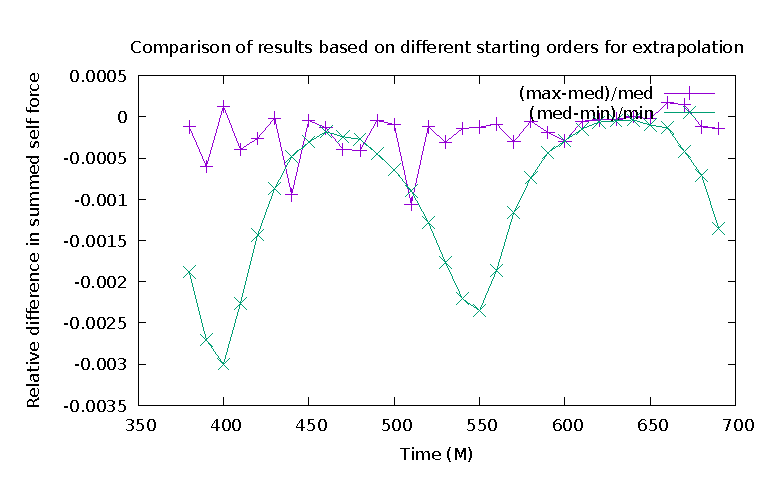
\includegraphics{minmaxmedrelativeerror3termavgl}
\end{figure}
\begin{figure}
  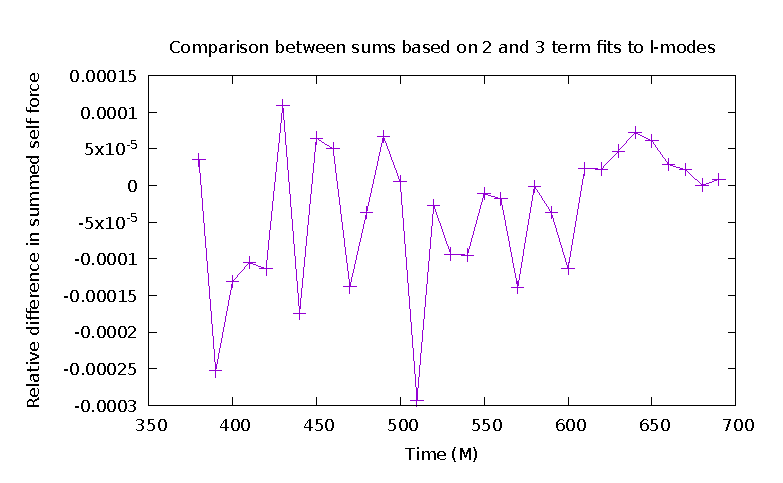
\includegraphics{relativeError23termSelfForce}
\end{figure}




\end{document}
